\documentclass[11pt,a4paper]{article}
\usepackage[margin=19mm,headheight=15pt,headsep=8mm,footskip=10mm]{geometry}
\usepackage[T1]{fontenc}
\usepackage[utf8]{inputenc}
\usepackage{lmodern}
\renewcommand{\familydefault}{\sfdefault}
\usepackage{microtype,graphicx,booktabs,tabularx,array,enumitem,xcolor}
\usepackage{tikz}
\usetikzlibrary{arrows.meta,positioning}
\usepackage{fancyhdr,hyperref}
\definecolor{ink}{HTML}{24394A}
\definecolor{blue}{HTML}{37657B}
\definecolor{pale}{HTML}{EDF3F6}
\definecolor{amber}{HTML}{A66E28}
\definecolor{cream}{HTML}{FAF3E7}
\hypersetup{colorlinks=true,linkcolor=blue,urlcolor=blue,pdftitle={BACE: Results and Discussion Brief},pdfsubject={Main experiment, five discussion points and source-inspected examples}}
\color{ink}
\setlength{\parindent}{0pt}
\setlength{\parskip}{6pt}
\setlength{\tabcolsep}{6pt}
\renewcommand{\arraystretch}{1.22}
\setlist[itemize]{leftmargin=15pt,itemsep=4pt,topsep=3pt}
\setlist[enumerate]{leftmargin=18pt,itemsep=6pt,topsep=3pt}
\pagestyle{fancy}
\fancyhf{}
\fancyhead[L]{\small\textcolor{blue}{BACE / RESULTS DISCUSSION}}
\fancyhead[R]{\small 8 October 2026}
\fancyfoot[L]{\footnotesize Working report \textbullet\ Automated results; independent validation pending}
\fancyfoot[R]{\thepage}
\renewcommand{\headrulewidth}{0.3pt}
\newcommand{\pagetitle}[2]{\textcolor{blue}{\small\bfseries #1}\par\vspace{2pt}{\LARGE\bfseries #2\par}\vspace{5pt}}
\newcommand{\lead}[1]{{\large\bfseries #1}\par}
\newcommand{\subhead}[1]{\vspace{5pt}\textbf{#1}\par}
\newcommand{\figcap}[2]{{\footnotesize\textbf{#1.} #2\par}}
\newcommand{\source}[1]{{\footnotesize\textcolor{blue}{Source: #1}\par}}
\newcommand{\callout}[2]{\par\vspace{4pt}\noindent\colorbox{pale}{\parbox{\dimexpr\linewidth-2\fboxsep\relax}{\vspace{4pt}\textbf{#1}\par #2\vspace{4pt}}}\par}
\newcommand{\question}[1]{\par\vspace{5pt}\noindent\colorbox{cream}{\parbox{\dimexpr\linewidth-2\fboxsep\relax}{\vspace{4pt}\textcolor{amber}{\textbf{For discussion}}\par #1\vspace{4pt}}}\par}
\newcommand{\quoted}[1]{\begin{quote}\small ``#1''\end{quote}}
\tikzset{box/.style={draw=blue!65,fill=pale,rounded corners=2pt,align=center,inner sep=7pt,font=\small},arrow/.style={-{Latex[length=2mm]},thick,draw=blue},notebox/.style={box,draw=amber!70,fill=cream}}
\begin{document}

\pagetitle{PART 1 / MAIN EXPERIMENT}{BACE: Results and Discussion Brief}
This report first summarizes the saved main experiment, then develops five discussion points using real project cases. The aim is to interpret the results and agree on the next validation steps.

\subhead{Study scope and what BACE measures}
The design includes \textbf{30 companies, five reporting years (2019--2023) and 12 ESRS tasks}. Of 1,800 planned company--year--task disclosures, \textbf{1,798} have complete BACE results and enter the native paired comparison. Two incomplete cases remain excluded, not scored as zero. Selection required source availability; this is not a representative sample of all companies.

\begin{center}
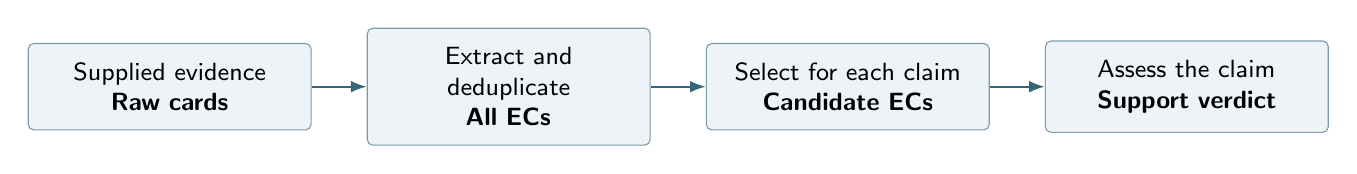
\begin{tikzpicture}
\node[box,text width=31mm] (cards) {Supplied evidence\\\textbf{Raw cards}};
\node[box,text width=31mm,right=7mm of cards] (ec) {Extract and deduplicate\\\textbf{All ECs}};
\node[box,text width=31mm,right=7mm of ec] (cand) {Select for each claim\\\textbf{Candidate ECs}};
\node[box,text width=31mm,right=7mm of cand] (judge) {Assess the claim\\\textbf{Support verdict}};
\draw[arrow] (cards)--(ec);\draw[arrow] (ec)--(cand);\draw[arrow] (cand)--(judge);
\end{tikzpicture}
\end{center}
{\small EC = evidence claim extracted from supplied material. DC = disclosure claim extracted from generated text. The support judge receives one DC, candidate ECs, company and target year.}

\begin{center}
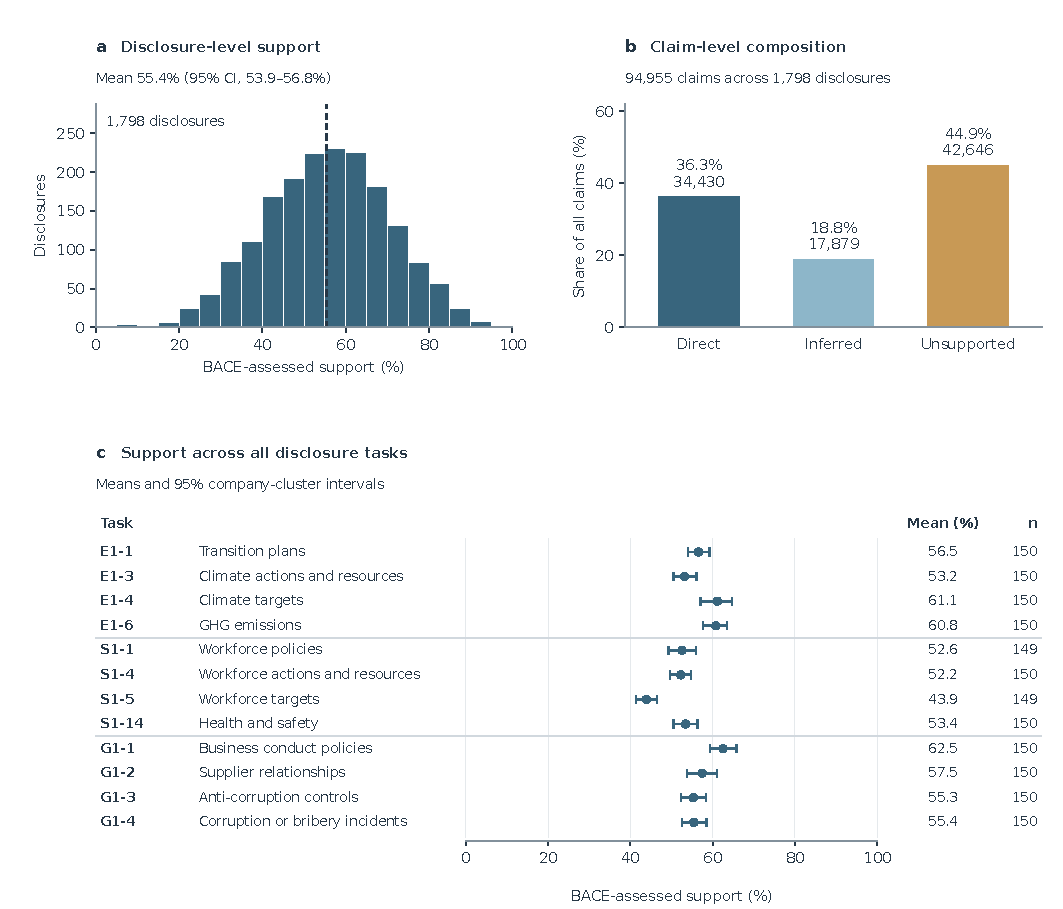
\includegraphics[width=0.91\linewidth,height=124mm,keepaspectratio]{assets/main_support.pdf}
\end{center}
\figcap{Figure 1}{Main-study support distribution, pooled claim composition and task means. Reproduced from manuscript Figure 2. The disclosure-macro mean is \textbf{55.4\%} (95\% company-cluster interval, 53.9--56.8\%). Of 94,955 DCs, 34,430 are direct, 17,879 inferred and 42,646 unsupported. Claim-pooled support is 55.1\%; it uses a different weighting.}
\source{Main snapshot; manuscript Figure 2 source data; numeric ledger, main/support and main/tasks.}

\newpage
\pagetitle{PART 1 / MAIN EXPERIMENT}{Three findings to take forward}
\textbf{Support varies across tasks.} Mean support ranges from \textbf{43.9\%} for workforce targets (S1-5) to \textbf{62.5\%} for business conduct policies (G1-1), descriptively.

\textbf{Two diagnoses dominate.} Factual boundary distortion and evidence conflation account for \textbf{73.5\%} of the 42,646 unsupported-claim diagnoses. These are mutually exclusive outputs of an ordered automated procedure.

\begin{center}\small\renewcommand{\arraystretch}{1.08}
\begin{tabularx}{0.94\linewidth}{Xrr}
\toprule
Automated diagnosis & Claims & Share of unsupported DCs\\
\midrule
Factual boundary distortion & 19,130 & 44.9\%\\
Evidence conflation & 12,205 & 28.6\%\\
Non-disclosure statement & 6,378 & 15.0\%\\
Inferential inflation & 3,193 & 7.5\%\\
Unsupported novelty & 1,698 & 4.0\%\\
Contradiction & 42 & 0.1\%\\
\bottomrule
\end{tabularx}\end{center}

\textbf{Native evaluator scores differ markedly.} Across the same 1,798 disclosures, means are \textbf{55.4\% for BACE, 90.2\% for RAGChecker and 90.7\% for RAGAS}. BACE is lower by 34.9 and 35.3 percentage points (pp), respectively.

\begin{center}
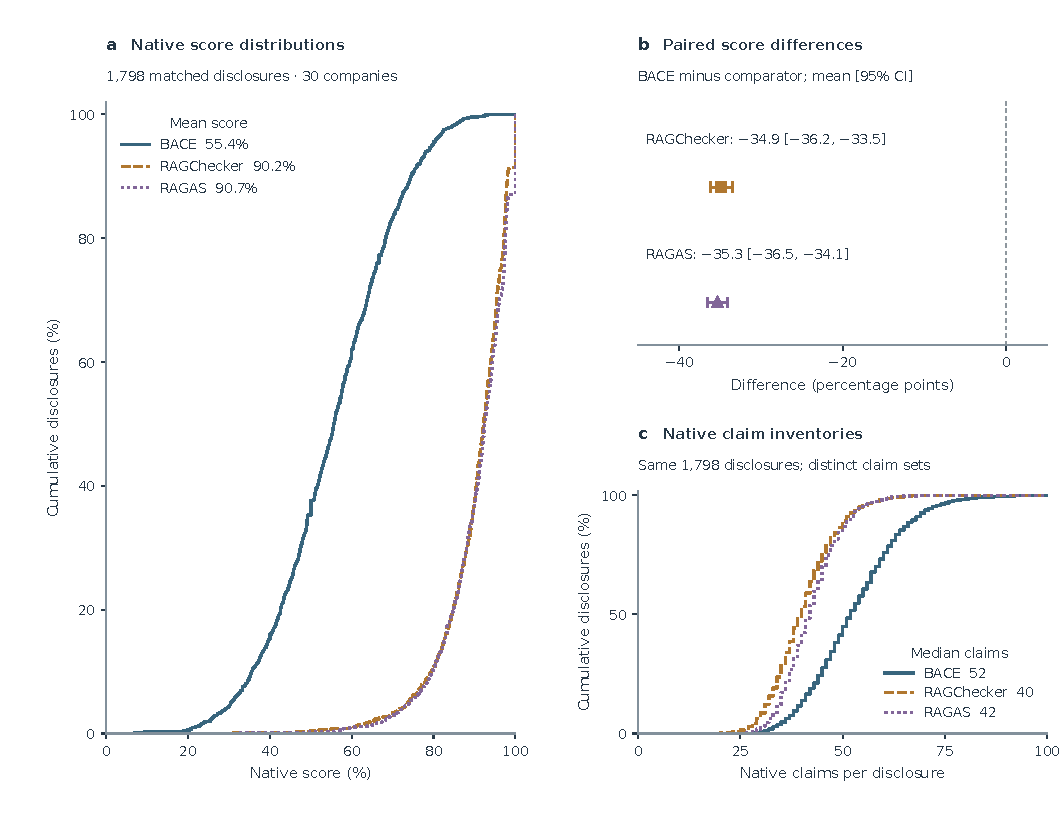
\includegraphics[width=0.94\linewidth,height=113mm,keepaspectratio]{assets/native_comparison.pdf}
\end{center}
\figcap{Figure 2}{Native score distributions, paired differences and claim inventories. Reproduced from manuscript Figure 4. Intervals resample companies. Native inventories differ: median claim counts are 52, 40 and 42. Pairing disclosures does not align their propositions.}
\textbf{Interpretation.} These automated assessments do not establish a factual-error rate, legal compliance or an evaluator accuracy ranking.
\source{Main snapshot; diagnosis composition; paired native differences; numeric ledger, main/diagnoses and main/comparators.}

\newpage
\pagetitle{PART 2 / DISCUSSION POINT 1}{What does the low support rate measure?}
\lead{An unsupported verdict is conditional on the evidence that reaches the judge.}

The main mean of 55.4\% summarizes BACE's judgments after evidence extraction, deduplication and candidate selection. A rejection can reflect an unsupported generated assertion, an altered evidence representation, an omitted premise, or a disputed judgment rule. The aggregate score does not distinguish these explanations.

\subhead{Real case C1: ASML, 2019 emissions disclosure}
The generated passage says:
\quoted{ASML's Scope 1 footprint has historically been defined as emissions from the combustion of natural gas and purchased CO\textsubscript{2}.}
BACE's extracted DC retained the purchased-CO\textsubscript{2} assertion. It returned \textbf{unsupported}, followed by a \textbf{contradiction} diagnosis. The diagnosis relied on an EC describing Scope 1 emissions through electricity consumption and local conversion factors.

\begin{center}
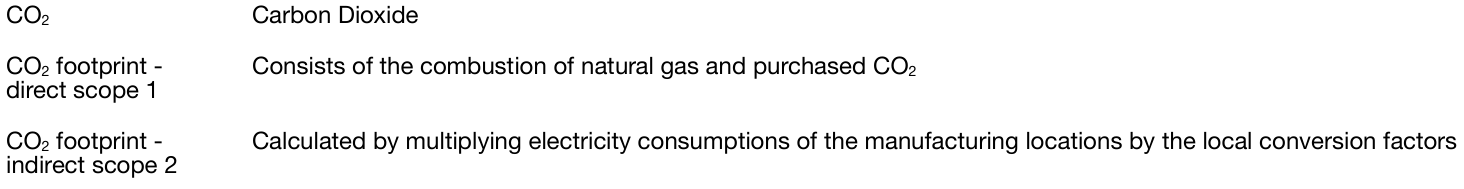
\includegraphics[width=0.98\linewidth]{assets/asml_glossary.png}
\end{center}
\figcap{Figure 3}{Original ASML Integrated Report 2018 glossary, printed p.~209 / PDF p.~216. Natural-gas combustion and purchased CO\textsubscript{2} belong to direct Scope 1; electricity and conversion factors belong to indirect Scope 2. The original row associations challenge the extracted EC.}

\begin{center}
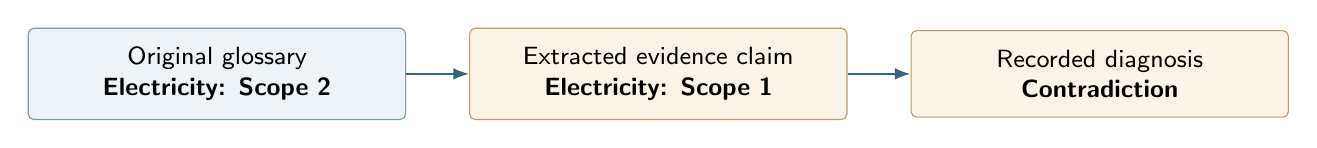
\begin{tikzpicture}
\node[box,text width=43mm] (source) {Original glossary\\\textbf{Electricity: Scope 2}};
\node[notebox,text width=43mm,right=8mm of source] (extract) {Extracted evidence claim\\\textbf{Electricity: Scope 1}};
\node[notebox,text width=43mm,right=8mm of extract] (verdict) {Recorded diagnosis\\\textbf{Contradiction}};
\draw[arrow] (source)--(extract);\draw[arrow] (extract)--(verdict);
\end{tikzpicture}
\end{center}

\subhead{What this example establishes}
Inspection of the original page exposes a row-association problem and challenges the recorded contradiction rationale. The supplied card had flattened the glossary, and the extracted EC attached the electricity definition to Scope 1. This is a concrete limitation in the evidence-processing chain.

\subhead{What it does not establish}
It does not validate every statement in the generated disclosure or determine how often this problem occurs. Diagnosis is produced after the support decision; its rationale is not a causal record of why the earlier support judge rejected the claim.

\question{How should we distinguish unsupported generated content from evidence-processing and judgment problems when interpreting the 55.4\% mean? Independent review should inspect the source representation as well as the final verdict.}
\source{C1 in case\_evidence.json; original report page and hash in original\_source\_checks.json. Original page rechecked on 8 October 2026.}

\newpage
\pagetitle{PART 2 / DISCUSSION POINT 2}{What do the dominant diagnoses mean?}
\lead{A boundary diagnosis can identify an unresolved reporting assumption.}

Boundary distortion and evidence conflation dominate the automated labels, but the labels are not independently confirmed error mechanisms. A key question is whether the judgment rules appropriately preserve time, population, units and relationships between facts.

\subhead{Real case C2: W\"artsil\"a, 2022 supplier-relationships disclosure}
The supplied evidence includes this passage from the 2019 annual report:
\quoted{W\"artsil\"a uses an online solution for supply chain risk identification, assessment, and monitoring.}
The generated 2022 disclosure contains the extracted claim:
\quoted{W\"artsil\"a uses an online solution for supply-chain risk identification.}
The selected EC explicitly attributes the use to 2019. BACE returns \textbf{unsupported} and assigns \textbf{factual boundary distortion}, because the historical observation does not establish use in the target year.

\begin{center}
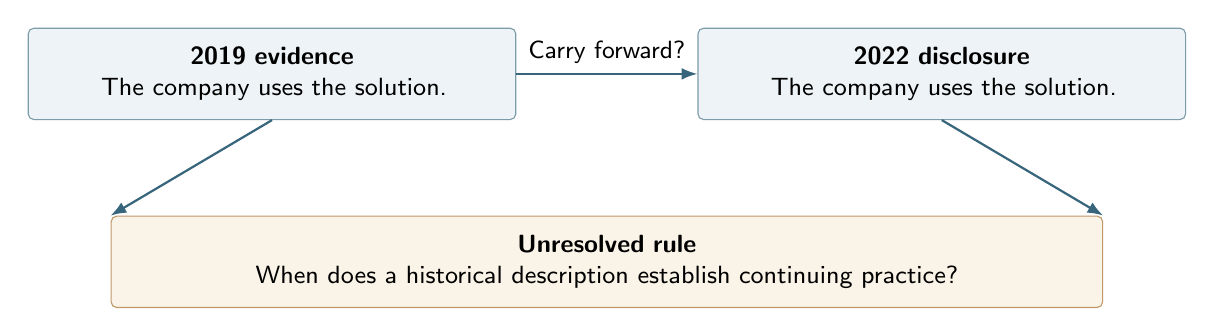
\begin{tikzpicture}
\node[box,text width=57mm] (past) {\textbf{2019 evidence}\\The company uses the solution.};
\node[box,text width=57mm,right=23mm of past] (current) {\textbf{2022 disclosure}\\The company uses the solution.};
\draw[arrow] (past)--node[above,font=\small]{Carry forward?}(current);
\path (past)--(current) coordinate[midway] (mid);
\node[notebox,text width=121mm,below=18mm of mid] (rule) {\textbf{Unresolved rule}\\When does a historical description establish continuing practice?};
\draw[arrow] (past.south)--(rule.north west);
\draw[arrow] (current.south)--(rule.north east);
\end{tikzpicture}
\end{center}

\subhead{Why the study design makes this important}
For reporting year $t$, the protocol supplies PDF report years $t-4$ through $t-1$, while structured metric years may include $t$. Historical PDF descriptions are therefore part of the intended evidence window. The same sentence can be read as a description of a continuing policy or as an assertion requiring current-year confirmation.

\subhead{What this example establishes}
The source documents the practice in 2019. It does \emph{not} establish that the practice stopped before 2022. The disagreement concerns the justification for temporal carry-forward, not observed discontinuation. This single temporal example also cannot identify the temporal share of the entire boundary-distortion category.

\question{Should historical policy and process descriptions support current-year statements by default, require explicit continuity evidence, or receive an uncertainty label? The rule should be stated before judging further examples and applied consistently across evaluators.}
\source{C2 in case\_evidence.json; supplied Evidence 7; W\"artsil\"a Annual Report 2019, p.~132. The local PDF contains selected annual-report elements. Original passage rechecked on 8 October 2026.}

\newpage
\pagetitle{PART 2 / DISCUSSION POINT 3}{How should evaluator disagreement be read?}
\lead{Inspect the proposition and its supporting evidence before comparing scores.}

The roughly 35-pp native gap is substantial, but different claim inventories and checking contexts prevent an accuracy ranking. Median native inventories are 52 BACE claims, 40 RAGChecker claims and 42 RAGAS claims per disclosure. A concrete disagreement can nevertheless expose the exact factual distinction at issue.

\subhead{Real case C3: SCA, 2022 corruption-and-bribery disclosure}
The supplied structured indicator is:
\quoted{Number of confirmed incidents in which own workers were dismissed or disciplined for corruption or bribery-related incidents.}
Its supplied value is \textbf{5.0}. The generated disclosure instead says:
\quoted{In connection with these incidents, five own workers were dismissed or subjected to disciplinary measures.}

\begin{center}
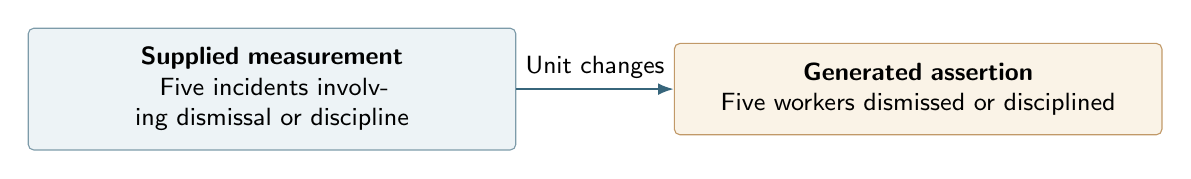
\begin{tikzpicture}
\node[box,text width=57mm] (inc) {\textbf{Supplied measurement}\\Five incidents involving dismissal or discipline};
\node[notebox,text width=57mm,right=20mm of inc] (workers) {\textbf{Generated assertion}\\Five workers dismissed or disciplined};
\draw[arrow] (inc)--node[above,font=\small]{Unit changes}(workers);
\end{tikzpicture}
\end{center}

\begin{center}
\begin{tabularx}{0.93\linewidth}{lX}
\toprule
Evaluator & Saved judgment on the worker-count proposition\\
\midrule
BACE & Unsupported; factual boundary distortion\\
RAGChecker & Supported\\
RAGAS & Supported\\
\bottomrule
\end{tabularx}
\end{center}

\subhead{What this example establishes}
An incident count does not determine the number of distinct workers involved. Both comparators retained the worker-count proposition and marked it supported; BACE rejected it. The supplied indicator does not establish the generated worker count. This is a traceable, source-relative disagreement about a measurement unit.

\subhead{What it does not establish}
The example does not verify SCA's real-world misconduct history or the correctness of the underlying extracted indicator. Nor does one selected disagreement establish comparative evaluator accuracy or representative error frequencies. The relevant source for this claim is the input indicator actually supplied to the models.

\question{Can an independent review compare the same complete propositions against the same evidence, including units and populations? Include disagreements in both directions so the validation does not assume that BACE is correct.}
\source{C3 in case\_evidence.json; supplied Evidence 23 and 26; RAGChecker claim index 25 and RAGAS statement index 31 (zero-based). Full supplied evidence and generated text are preserved in the case bundle.}

\newpage
\pagetitle{PART 2 / DISCUSSION POINT 4}{How much do judgment instructions matter?}
\lead{Fixed claims and evidence still produce different support judgments.}

The prompt experiment fixes DCs, candidate ECs, model settings and the output task, changing only the judgment instructions. It analyses \textbf{1,796 complete disclosures and 94,854 claims}; three failed records exclude two whole disclosures.

\begin{center}\small
\begin{tabularx}{\linewidth}{Xrr}
\toprule
Condition within BACE & Mean support & Change from original\\
\midrule
Original instructions & 55.36\% & Reference\\
RAGAS-style instructions & 63.02\% & +7.66 pp\\
RAGChecker-style instructions & 60.34\% & +4.97 pp\\
\bottomrule
\end{tabularx}
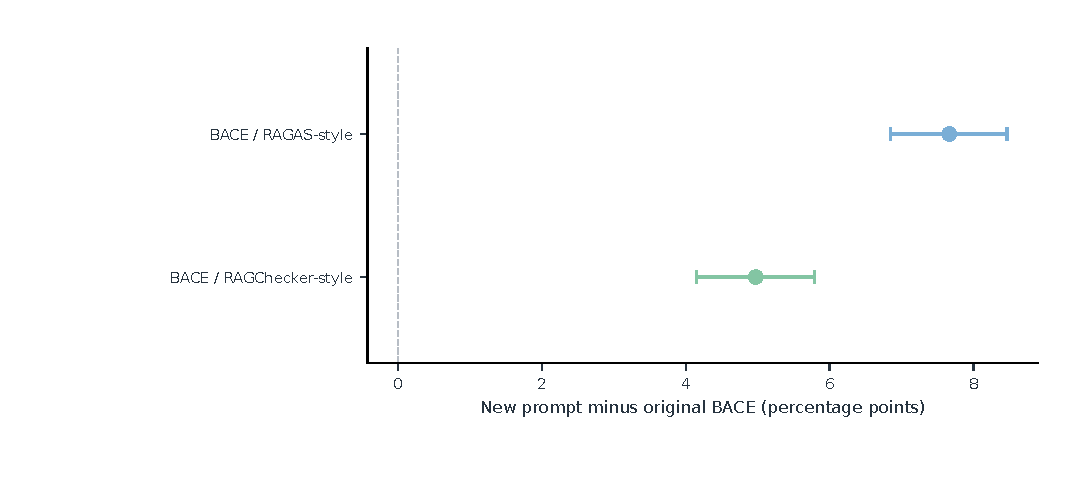
\includegraphics[width=0.91\linewidth,height=58mm,keepaspectratio,trim=75bp 26bp 15bp 18bp,clip]{assets/prompt_effects.pdf}
\end{center}
\figcap{Figure 4}{Paired changes under adapted instructions. Saved 95\% company-cluster intervals are +6.84 to +8.46 pp and +4.14 to +5.79 pp. The variants retain BACE's support-set task; they are not native comparator reruns.}

\subhead{Real case C4: Kinnevik, 2020 business-conduct disclosure}
The fixed target is:
\quoted{Kinnevik's Code of Conduct addresses anti-bribery.}
All four candidate ECs describe anti-bribery provisions in the \textbf{2017 or 2018} reports, while the target year is \textbf{2020}.

\textbf{Saved judgments:} original = unsupported; RAGAS-style = unsupported; RAGChecker-style = supported.

\subhead{Interpretation and limit}
The same target and candidates yield different outcomes. Temporal interpretation is a plausible issue, not an established cause: support outputs contain sets rather than prose rationales. Both variants also remove support from other claims, so neither is a uniform relaxation.

On a fixed 60-disclosure repeat subset, rerunning the original instructions changes the mean by only $-0.49$ pp, while \textbf{9.95\% of claims flip}. Individual changes cannot all be assigned to prompt changes. One repeat does not estimate all run variability.

\question{Which temporal and inference rules should be explicit and held constant? Validate the changed judgments before interpreting higher support as improvement, and do not allocate the native evaluator gap to this prompt effect.}
\source{C4 in case\_evidence.json; prompt experiment scores, effects, repeat transitions and frozen protocol.}

\newpage
\pagetitle{PART 2 / DISCUSSION POINT 5}{How much does evidence selection matter?}
\lead{Changing the supplied evidence changes support, but not necessarily through omission.}

The evidence-chain experiment selected 90 disclosures, one per company--E/S/G stratum. One failed record excludes one disclosure, leaving \textbf{89 paired disclosures and 4,746 DCs across 30 companies}. Targets, model settings and the common BACE judgment criterion are fixed. Each condition is judged separately.

\begin{center}
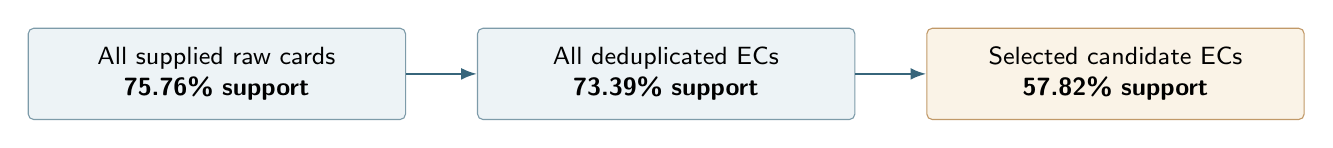
\begin{tikzpicture}
\node[box,text width=43mm] (raw) {All supplied raw cards\\\textbf{75.76\% support}};
\node[box,text width=43mm,right=9mm of raw] (all) {All deduplicated ECs\\\textbf{73.39\% support}};
\node[notebox,text width=43mm,right=9mm of all] (cand) {Selected candidate ECs\\\textbf{57.82\% support}};
\draw[arrow] (raw)--(all);\draw[arrow] (all)--(cand);
\end{tikzpicture}
\end{center}
\figcap{Figure 5}{Evidence-processing stages and their separately measured sampled-cohort macro rates. Arrows show the processing sequence, not validated evidence-loss rates. Raw cards are the original prompt-visible material, not complete PDFs.}

\begin{center}\small
\begin{tabularx}{\linewidth}{Xrr}
\toprule
Paired contrast & Difference & 95\% cluster interval\\
\midrule
Raw cards minus all ECs & +2.37 pp & +0.27 to +4.36\\
All ECs minus candidates & +15.58 pp & +13.72 to +17.50\\
Raw cards minus candidates & +17.94 pp & +15.81 to +19.92\\
\bottomrule
\end{tabularx}
\end{center}

\subhead{Real case C5: DiaSorin, 2023 business-conduct disclosure}
The fixed target is ``DiaSorin's periodic training addresses Legislative Decree 231/2001.'' The sole candidate EC states:
\quoted{According to DiaSorin's 2022 annual report, the Group provides regular training activities on topics under Legislative Decree 231/2001 and the Model.}

\begin{center}\small
\begin{tabularx}{\linewidth}{lXl}
\toprule
Input condition & Recorded support set & Verdict\\
\midrule
30 raw cards & Card 9: the training passage & Supported\\
78 ECs & EC 76 alone: the quoted EC above & Supported\\
1 candidate EC & EC 76 is supplied; output set is empty & Unsupported\\
\bottomrule
\end{tabularx}
\end{center}

\subhead{Why this is an important counterexample}
The full-EC condition accepts \textbf{the very EC retained in the candidate condition}. That EC was not omitted. The case therefore demonstrates a judgment change associated with context/run conditions, rather than proving candidate evidence loss. Whether the 2022 description supports the 2023 assertion remains a separate temporal question.

The larger aggregate contrast makes candidate selection and context a priority for review. However, more evidence can change judge behavior without adding a necessary premise. The 15.58-pp difference is not a measured loss rate, and this sampled-cohort result must not replace the main-study mean or be added to the prompt effect.

\question{For changed judgments, is a necessary premise actually missing, or does the model judge the same premise differently in a larger context? Independent review must distinguish these possibilities.}
\source{C5 in case\_evidence.json; three original call records; supplied Card 9; DiaSorin Annual Report 2022, PDF p.~201; sampled scores and effects.}

\newpage
\pagetitle{PART 3 / DECISIONS AND SOURCES}{What should the meeting decide?}

\begin{enumerate}
\item \textbf{Agree on the claim the paper can currently defend.} The study documents evidence-support patterns, concrete boundary disagreements and sensitivity to instructions and evidence inputs. Comparative accuracy remains unresolved.
\item \textbf{Prioritize independent review of the full evidence chain.} Check whether the DC represents the generated passage, whether the supplied cards support it, whether the EC pool preserves the necessary premises, and whether candidates retain them. Include both support additions and removals and preserve uncertainty.
\item \textbf{Specify temporal and inference rules.} Decide when historical policies support current statements and which combinations of separately evidenced facts are sufficient. Apply the rules consistently before interpreting new judgments.
\item \textbf{Update the manuscript around the completed work.} Integrate the prompt and sampled evidence-chain experiments into Results and Methods. The existing four manuscript main figures do not yet include these extensions.
\end{enumerate}

\subhead{Current validation and statistical boundaries}
The local formal reviewer A/B workbooks each contain 600 sample rows and remain unchanged from the inspected blank versions. They assess judgments conditional on supplied DCs and candidate ECs, not the entire upstream pipeline. The separate evidence-chain packet contains 160 review rows and no completed local annotations.

All macro rates give each complete disclosure equal weight; claim-pooled proportions are labelled separately. Saved 95\% percentile intervals use 2,000 company-cluster bootstrap draws, seed 20260921. They condition on observed model outputs and do not measure all model-run or annotation uncertainty. The sampled evidence-chain intervals are not exact finite-population intervals for the full 1,798-disclosure frame. The original full evidence-chain run was stopped for sampling.

\subhead{Case and source guide}
\begin{center}\footnotesize
\begin{tabularx}{\linewidth}{l l X}
\toprule
ID & Case & Exact source locator and scope\\
\midrule
C1 & ASML, 2019 & Main run, E1-6; supplied Evidence 2; original 2018 glossary, PDF p.~216 / printed p.~209. Challenges a diagnosis rationale.\\
C2 & W\"artsil\"a, 2022 & Main run, G1-2; supplied Evidence 7; 2019 report p.~132. Historical-to-current interpretation.\\
C3 & SCA, 2022 & Main run, G1-4; supplied indicators 23 and 26; comparator indices 25 / 31. Incidents versus distinct workers.\\
C4 & Kinnevik, 2020 & Prompt experiment, G1-1; DC ending \texttt{45dea2}; four fixed ECs from 2017/2018 reports. No independent correctness label.\\
C5 & DiaSorin, 2023 & Sampled evidence-chain experiment, G1-1; review ID \texttt{review\_c109416f135da65f}; EC 76 and raw Card 9. Same accepted EC retained in rejected candidate condition.\\
\bottomrule
\end{tabularx}
\end{center}

\textbf{Companion files.} The \href{case_evidence.json}{case evidence ledger} preserves full IDs, supplied evidence and judgments. \href{original_source_checks.json}{Original-source checks} record PDF passages, versions and access dates. The \href{numeric_ledger.json}{numeric ledger} records cohorts and estimates; \href{provenance.json}{provenance} records input hashes and verification scope. The \href{REPORT_PLAN.md}{report plan} preserves the outline.

\textbf{Review scope.} All five examples are real saved project cases, selected for explanation. Source and call inspection for this report is an assistant analysis, not independent human validation or a representative error audit. Original PDF checks do not expand the evidence that was supplied during evaluation. No experiments or frozen artifacts were changed.
\end{document}
